\documentclass{article}

\usepackage{caption}
\usepackage{amsmath, amssymb, amsfonts}
\usepackage{amsthm}
\usepackage{tikz}
\usepackage{thmtools}
\usepackage{graphicx}
\usepackage{setspace}
\usepackage{geometry}
\usepackage{float}
\usepackage{hyperref}
\usepackage[utf8]{inputenc}
\usepackage[english]{babel}
\usepackage{framed}
\usepackage{tcolorbox}
\usepackage{comment}
\usepackage{titlesec}
\usepackage{enumitem}
\usepackage{array}
\usepackage{multirow, bigdelim}
\usepackage{marginnote}
\usepackage{lipsum}
\usepackage{neuralnetwork}
\usepackage{subfigure}
\usepackage{slashed}

\usetikzlibrary{graphs}
\usetikzlibrary{shapes}
\usetikzlibrary{backgrounds}
\usetikzlibrary{calc}
\usetikzlibrary{patterns}
\usetikzlibrary{positioning, fit, arrows.meta}

\newenvironment{solution}{\textit{Solution}.}

\titleformat{\subsection}[block]{\normalfont\Large\bfseries}{\thesubsection}{1em}{}
\titleformat{\subsubsection}[hang]{\normalfont\bfseries}{}{1em}{}

%%% Problem Numbering and Formatting

\def \proofDistance {5pt}
\def \subheaderSpace {10pt}


%%% PAGE DIMENSIONS
\usepackage{geometry} % to change the page dimensions
\geometry{margin=1in} % for example, change the margins to 1 inches all round

\newcommand{\proofseparator}{\par\noindent\rule{\textwidth}{0.4pt}}
\newcommand{\caution}{\marginnote{
\includegraphics[width=2em]{caution.png}}}
\newcommand{\HRule}[1]{\rule{\linewidth}{#1}}


% Natural Numbers 
\newcommand{\N}{\ensuremath{\mathbb{N}}}

% Whole Numbers
\newcommand{\W}{\ensuremath{\mathbb{W}}}

% Integers
\newcommand{\Z}{\ensuremath{\mathbb{Z}}}

% Rational Numbers
\newcommand{\Q}{\ensuremath{\mathbb{Q}}}

% Real Numbers
\newcommand{\R}{\ensuremath{\mathbb{R}}}

% Complex Numbers
\newcommand{\C}{\ensuremath{\mathbb{C}}}

% Command for problem statement
\newcommand{\pb}[1]{
    \begin{problem}
    #1
    \end{problem}
}

% Define a command for custom proofs with separator
\newcommand{\pf}[1]{
    \vspace{\proofDistance}
    \begin{proof}
    #1
    \end{proof}
    \proofseparator
}

\newcommand{\sol}[1]{
    \vspace{\proofDistance}
    \begin{solution}
    #1
    \end{solution}
    \proofseparator
}

\newcommand{\makespace}[1]{\vspace{\subheaderSpace}}

\titleformat*{\section}{\Large\bfseries}
\titleformat*{\subsection}{\large\bfseries}

% ------------------------------------------------------------------------------

\begin{document}

% ------------------------------------------------------------------------------
% Cover Page and ToC
% ------------------------------------------------------------------------------

\title{ \normalsize \textsc{}
		\\ [2.0cm]
        \HRule{1.5pt} \\
		\LARGE \textbf{\uppercase{DISCRETE MATHEMATICS}
		\HRule{2.0pt} \\ [0.6cm] \LARGE{Writing Assignment 2} \vspace*{10\baselineskip}}
		}
\date{2nd Semester, 2024}
\author{\textbf{Authors} \\ 
		Paul Beggs, Thomas Sebring}

\maketitle
\newpage

% ------------------------------------------------------------------------------
% Introduction
% ------------------------------------------------------------------------------
\section{Overview}

    Computational efficiency is not just a technical necessity but a pivotal factor that determines the practicality of algorithms across various applications. Thus, we aim to show that as the complexity of problems tackled by modern computers escalates, understanding how the size of an input impacts the time required to compute an output becomes crucial.
    
    In this writing assignment, we will delve into this intricate relationship by examining the time complexity of various algorithms as a function of their input sizes. Specifically, for an input of size $n$, we will show there is a relationship between $n$ and the time it takes to run, denoted as $t(n)$. Hence, we will transform theoretical functions into computational experiments by utilizing $\log$-$\log$ plots to discern patterns and predict performance. This will allow us to analyze a set of distinct algorithms—ranging from simple linear searches to complex matrix operations—each chosen to illuminate unique aspects of computational behavior as the input size scales. 
    
    Through analysis of varying function types, we will show a table for $\ln(n)$ and $\ln(f(n))$ for each $n = 20, 25, 30, 35, 40, 45, 50, 55, 60$, then plot these points on a scatter plot. This will give us an idea for how the size of the input is related to the time needed for each algorithm (where $\ln(f(n))$ is representative of the amount of time needed). Then, we will evaluate computer science algorithms that are derived from these function types. Thus, by the end of this report, we aim to present a comprehensive overview that not only addresses the hows and whys of algorithm performance relative to input sizes but also enhances our collective understanding of mathematical concepts applied in a computational context.

% ------------------------------------------------------------------------------
% Body
% ------------------------------------------------------------------------------

\section{Notable Functions}

    \subsection{Polynomial Growth}

    As depicted in the results (refer to Tables 1-3 and Figures 1-3), a clear trend emerges indicating that as the number of items, represented by $n$, increases, there is a notable decrease in the relative amount of time needed between successive values of $n$. This phenomenon suggests a diminishing marginal increase in processing time as the dataset grows. Specifically, the incremental time required to process additional elements becomes smaller. This observation might seem counter-intuitive, as one might expect larger datasets to require proportionally more time. However, from these results obtained from the provided polynomial functions, we can see that this is not the case. 

    \subsubsection{Linear}

\noindent
\begin{minipage}{0.3\textwidth} % Sets the minipage to take up half of the page
    \centering

    
    
    \begin{tabular}{c|c|c}
        $n$ & $\ln(n)$ & $\ln(f(n))$ \\ \hline
        20 & $2.995$ & $4.11$ \\\hline
        25 & $3.218$ & $4.33$  \\\hline
        30 & $3.401$ & $4.51$\\\hline
        35 & $3.555$ & $4.663$\\\hline
        40 & $3.688$ & $4.795$\\ \hline
        45 & $3.806$ & $4.912$\\ \hline
        50 & $3.912$ & $5.017$\\ \hline
        55 & $4.007$ & $5.111$\\ \hline
        60 & $4.094$ & $5.198$\\
    \end{tabular}

    
    
    \captionof{table}{$f(n) = 3n + 1$} % Caption goes in the curly braces. Replace "Your Table Caption."
\end{minipage}%
\begin{minipage}{0.6\textwidth} % See above for reference

    

    \centering
    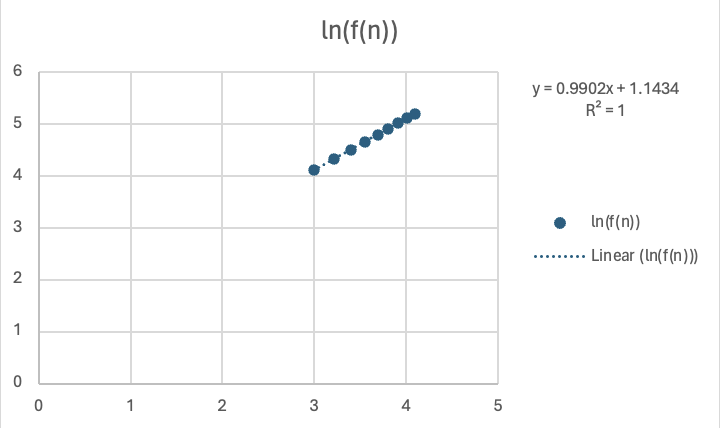
\includegraphics[width=1\linewidth]{Graphs/3n+1.png} % If the image is too large, change the "width=1" to something smaller. 
    \captionof{figure}{$f(n) = 3n + 1$}

     
    
\end{minipage}

    \subsubsection{Quadratic}


\noindent
\begin{minipage}{0.3\textwidth} % Sets the minipage to take up half of the page
    \centering

    
    
    \begin{tabular}{c|c|c}
        $n$ & $\ln(n)$ & $\ln(f(n))$ \\ \hline
        20 & $2.995$ & $6.758$ \\\hline
        25 & $3.218$ & $7.189$  \\\hline
        30 & $3.401$ & $7.544$\\\hline
        35 & $3.555$ & $7.846$\\\hline
        40 & $3.688$ & $8.108$\\ \hline
        45 & $3.806$ & $8.339$\\ \hline
        50 & $3.912$ & $8.546$\\ \hline
        55 & $4.007$ & $8.734$\\ \hline
        60 & $4.094$ & $8.906$\\
    \end{tabular}

    
    
    \captionof{table}{$f(n)=2n^2+3n+1$} % Caption goes in the curly braces. Replace "Your Table Caption."
\end{minipage}%
\begin{minipage}{0.6\textwidth} % See above for reference

    

    \centering
    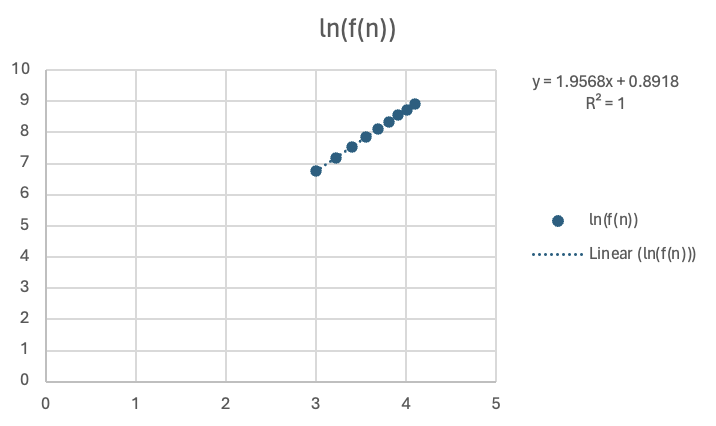
\includegraphics[width=1\linewidth]{Graphs/2n^2+3n+1.png} % If the image is too large, change the "width=1" to something smaller. 
    \captionof{figure}{$f(n)=2n^2+3n+1$}

     
    
\end{minipage}\noindent

    \subsubsection{Quintic}

\begin{minipage}{0.3\textwidth} % Sets the minipage to take up half of the page
    \centering

    
    
    \begin{tabular}{c|c|c}
        $n$ & $\ln(n)$ & $\ln(f(n))$ \\ \hline
        20 & $2.995$ & $14.998$ \\\hline
        25 & $3.218$ & $16.107$  \\\hline
        30 & $3.401$ & $17.014$\\\hline
        35 & $3.555$ & $17.783$\\\hline
        40 & $3.688$ & $18.449$\\ \hline
        45 & $3.806$ & $19.037$\\ \hline
        50 & $3.912$ & $19.563$\\ \hline
        55 & $4.007$ & $20.039$\\ \hline
        60 & $4.094$ & $20.473$\\
    \end{tabular}

    
    
    \captionof{table}{$f(n) = n^5 + 8n^3 + n$} % Caption goes in the curly braces. Replace "Your Table Caption."
\end{minipage}%
\begin{minipage}{0.6\textwidth} % See above for reference

    

    \centering
    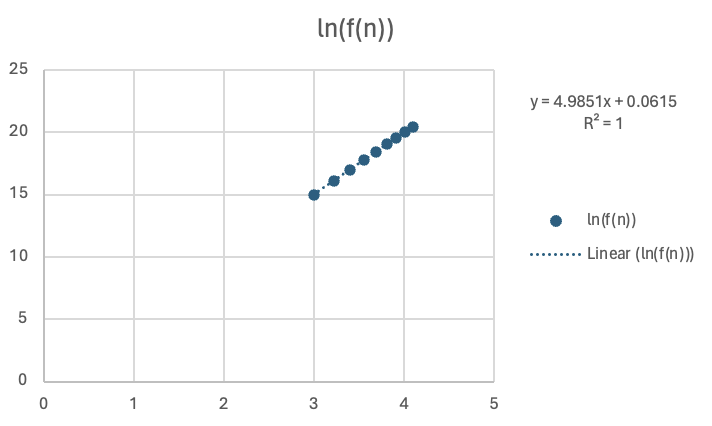
\includegraphics[width=1\linewidth]{Graphs/n^5+8n^3+n.png} % If the image is too large, change the "width=1" to something smaller. 
    \captionof{figure}{$f(n) = n^5 + 8n^3 + n$}

     
    
\end{minipage}\noindent
\newpage
        \subsubsection{Exponential}

        Note for Table 4 we can see that the growth factor between $n$ terms \textit{appears} to be a constant growth rate. However, when we observe the $R^2$ value (see Figure 4), we see that is not exactly 1. Hence, if had a larger dataset, we would see the growth factor increase, rather than have diminishing returns such as the linear, quadratic, and quintic functions.


\begin{minipage}{0.3\textwidth} % Sets the minipage to take up half of the page
    \centering

    
    
    \begin{tabular}{c|c|c}
        $n$ & $\ln(n)$ & $\ln(f(n))$ \\ \hline
        20 & $2.995$ & $13.864$ \\\hline
        25 & $3.218$ & $17.328$  \\\hline
        30 & $3.401$ & $20.794$\\\hline
        35 & $3.555$ & $24.26$\\\hline
        40 & $3.688$ & $27.725$\\ \hline
        45 & $3.806$ & $31.191$\\ \hline
        50 & $3.912$ & $34.657$\\ \hline
        55 & $4.007$ & $38.123$\\ \hline
        60 & $4.094$ & $41.588$\\
    \end{tabular}

    
    
    \captionof{table}{$f(n) = 2^n + 5n^2 + 1$} % Caption goes in the curly braces. Replace "Your Table Caption."
\end{minipage}%
\begin{minipage}{0.6\textwidth} % See above for reference

    

    \centering
    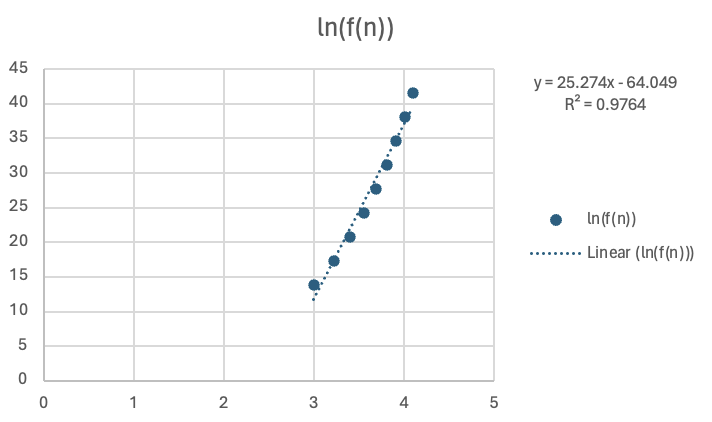
\includegraphics[width=1\linewidth]{Graphs/2^n+5n^2+1.png} % If the image is too large, change the "width=1" to something smaller. 
    \captionof{figure}{$f(n) = 2^n + 5n^2 + 1$}

     
    
\end{minipage}


    \subsection{Factorial}

    We can see a similar relationship between the terms for these factorial values that we saw for the exponential values. That is, if we know that $n!$ grows faster than $x^n$ from previous assignments, then we can hypothesize that the growth rate between these terms will also not be diminishing. In fact, we can prove this hypothesis by observing the $R^2$ value -- as we did with the exponential graph (see Figure 5). 


\begin{minipage}{0.3\textwidth} % Sets the minipage to take up half of the page
    \centering

    
    
    \begin{tabular}{c|c|c}
        $n$ & $\ln(n)$ & $\ln(f(n))$ \\ \hline
        20 & $2.995$ & $42.335$ \\\hline
        25 & $3.218$ & $58.003$  \\\hline
        30 & $3.401$ & $74.658$\\\hline
        35 & $3.555$ & $92.136$\\\hline
        40 & $3.688$ & $110.32$\\ \hline
        45 & $3.806$ & $129.123$\\ \hline
        50 & $3.912$ & $148.477$\\ \hline
        55 & $4.007$ & $168.327$\\ \hline
        60 & $4.094$ & $188.628$\\
    \end{tabular}

    
    
    \captionof{table}{$f(n) = n!$} % Caption goes in the curly braces. Replace "Your Table Caption."
\end{minipage}%
\begin{minipage}{0.6\textwidth} % See above for reference

    

    \centering
    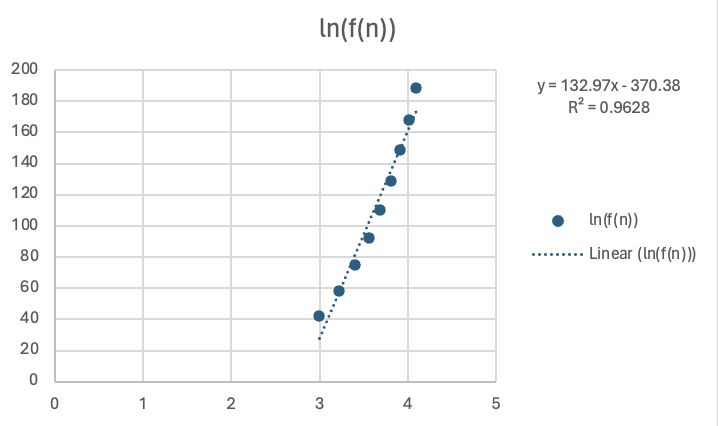
\includegraphics[width=1\linewidth]{Graphs/n!.png} % If the image is too large, change the "width=1" to something smaller. 
    \captionof{figure}{$f(n) = n!$}

     
    
\end{minipage}

\newpage

% ------------------------------------------------------------------------------
% Computational Algorithms
% ------------------------------------------------------------------------------

\section{Computational Algorithms}

    Computational algorithms are step-by-step procedures for solving problems, processing data, or conducting calculations. They serve as the backbone of all computer software, enabling everything from simple arithmetic operations to complex simulations and data analysis tasks. Algorithms are essential for designing efficient and effective software systems, as they specify the exact sequence of steps needed to perform a desired task.

    \subsection{Linear Search}

    

\begin{minipage}{0.4\textwidth} % Sets the minipage to take up half of the page
    \centering

    
    
    \begin{tabular}{c|c|c|c}
        $n$ & $\ln(n)$ & Time(s) & $\ln(f(n))$ \\ \hline
        5000 & $6.907$ & $0.137$ & $-1.986$ \\ \hline
        10000 & $8.517$ & $0.529$ & $-0.635$  \\ \hline
        20000 & $9.21$ & $2.131$ & $0.756$\\ \hline
        30000 & $10.308$ & $3.412$ & $1.227$\\ \hline
        40000 & $10.596$ & $4.677$ & $1.542$\\ \hline
        50000 & $10.819$ & $6.125$ & $1.812$\\ \hline
        60000 & $11.002$ & $8.052$ & $2.086$\\ \hline
        70000 & $11.156$ & $9.003$ & $2.197$\\ \hline
        80000 & $11.289$ & $10.086$ & $2.311$\\ \hline
        90000 & $11.407$ & $11.462$ & $2.439$\\ \hline
        100000 & $11.512$ & $13.886$ & $2.63$\\
    \end{tabular}
    
    \captionof{table}{Linear Search of $n$} % Caption goes in the curly braces. Replace "Your Table Caption."
\end{minipage}%
\begin{minipage}{0.6\textwidth} % See above for reference

    

    \centering
    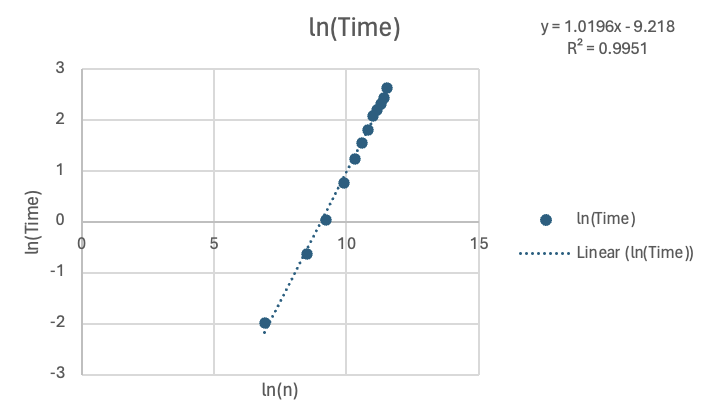
\includegraphics[width=1\linewidth]{Graphs/Linear.png} % If the image is too large, change the "width=1" to something smaller. 
    \captionof{figure}{Linear Search of $n$}

     
    
\end{minipage} \\

        \textit{Linear Search} is an algorithm that when given an unordered list of length $n$ and a target value $c$, it will determine if $c$ is in the list. This search method involves scanning each element of the list sequentially until the target is found or the list is fully traversed. Because of its straightforward nature, linear search does not require the list to be sorted, making it versatile for scenarios where data is dynamically altered or sorting is impractical. This $R^2$ score closely resembles that of the polynomial graph from Section 2.


    \subsection{Naive Sort}

    
    
\begin{minipage}{0.4\textwidth} % Sets the minipage to take up half of the page
    \centering

    
    
    \begin{tabular}{c|c|c|c}
        $n$ & $\ln(n)$ & Time(s) & $\ln(f(n))$ \\ \hline
        100 & $4.605$ & $0.119$ & $-2.121$ \\\hline
        200 & $5.298$ & $0.479$ & $-0.734$  \\\hline
        500 & $6.214$ & $3.199$ & $1.163$\\\hline
        750 & $6.620$ & $7.321$ & $1.99$\\\hline
        1000 & $6.907$ & $14.261$ & $2.657$\\ \hline
        1250 & $7.13$ & $20.57$ & $3.023$\\ \hline
        1500 & $7.313$ & $30.524$ & $3.418$\\ \hline
        2000 & $7.6$ & $55.764$ & $4.021$\\ \hline
        2500 & $7.824$ & $87.796$ & $4.475$\\
    \end{tabular}
    
    \captionof{table}{Naive Sort of $n$} % Caption goes in the curly braces. Replace "Your Table Caption."
\end{minipage}%
\begin{minipage}{0.6\textwidth} % See above for reference

    

    \centering
    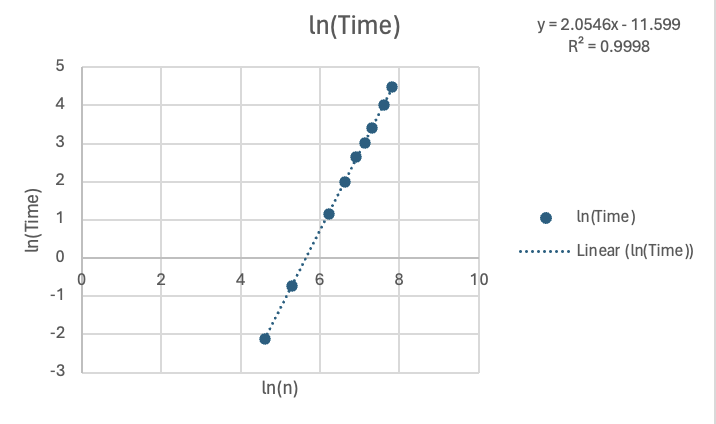
\includegraphics[width=1\linewidth]{Graphs/Naive.png} % If the image is too large, change the "width=1" to something smaller. 
    \captionof{figure}{Naive Sort of $n$}

\end{minipage} \\

        \textit{Naive Sort} works by giving an algorithm a random set of integers (of length $n$), and then sorting them by brute force. That is, it will compare one item in the list with its neighbor, and if that item is larger than it, they switch. This process repeats for every item in the list. This quadratic relationship between time and input size renders it impractical for large datasets. Similar to Linear search, we can see the $R^2$ score is almost exactly the same as the polynomial graphs from Section 2.

    \subsection{Python's \texttt{Sorted}}



    \begin{minipage}{0.4\textwidth} % Sets the minipage to take up half of the page
    \centering
    
    \begin{tabular}{c|c|c|c}
        $n$ & $\ln(n)$ & Time(s) & $\ln(f(n))$ \\ \hline
        100 & $4.605$ & $0.01$ & $-4.544$ \\\hline
        200 & $5.298$ & $0.012$ & $-4.421$  \\\hline
        500 & $6.214$ & $0.036$ & $-3.299$\\\hline
        750 & $6.620$ & $0.062$ & $-2.769$\\\hline
        1000 & $6.907$ & $0.113$ & $-2.172$\\ \hline
        1250 & $7.13$ & $0.231$ & $-1.463$\\ \hline
        1500 & $7.313$ & $0.288$  & $-1.244$\\ \hline
        2000 & $7.6$ & $0.415$ & $-0.877$\\ \hline
        2500 & $7.824$ & $0.545$ & $-0.605$\\
    \end{tabular}

    
    
    \captionof{table}{Python Sorting of $n$} % Caption goes in the curly braces. Replace "Your Table Caption."
\end{minipage}%
\begin{minipage}{0.6\textwidth} % See above for reference

    

    \centering
    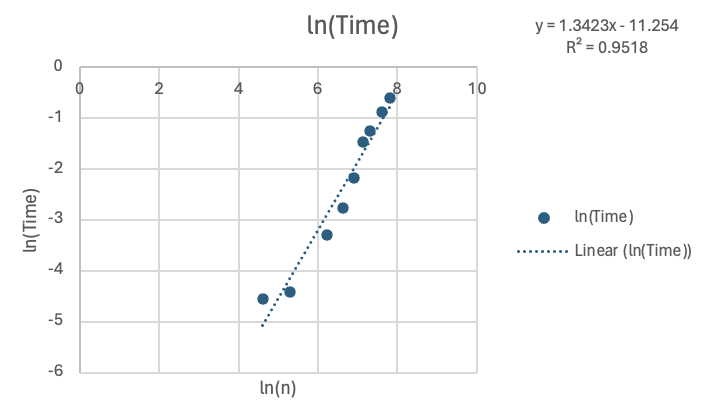
\includegraphics[width=1\linewidth]{Graphs/Python.png} % If the image is too large, change the "width=1" to something smaller. 
    \captionof{figure}{Python Sorting of $n$}

     
    
\end{minipage}\\

    \textit{Python's \texttt{Sorted}} is a built-in function that provides a highly optimized approach to sorting arrays and lists. This function is versatile, allowing for sorting based on natural ordering as well as via a custom key function. Python's \texttt{Sorted} uses an algorithm known as Timsort, which is a hybrid sorting algorithm derived from merge sort and insertion sort. The $R^2$ score resembles that of factorial graph from Section 2.2.

    \subsection{Matrix Determinant}

    

    \begin{minipage}{0.4\textwidth} % Sets the minipage to take up half of the page
    \centering

    
    
    \begin{tabular}{c|c|c|c}
        $n$ & $\ln(n)$ & Time(s) & $\ln(f(n))$ \\ \hline
        100 & $4.605$ & $1.159$ & $0.148$ \\\hline
        150 & $5.01$ & $2.775$ & $1.02$  \\\hline
        200 & $5.298$ & $5.062$ & $1.621$\\\hline
        250 & $5.521$ & $10.108$ & $2.313$\\\hline
        300 & $5.703$ & $13.547$ & $2.606$\\ \hline
        350 & $5.857$ & $21.927$ & $3.087$\\ \hline
        400 & $5.991$ & $30.317$ & $3.411$\\ \hline
        450 & $6.109$ & $42.876$ & $3.758$\\ \hline
        500 & $6.214$ & $55.179$ & $4.01$\\
    \end{tabular}

    
    \captionof{table}{\centering Matrix Determinant of $n$} % Caption goes in the curly braces. Replace "Your Table Caption."
\end{minipage}%
\begin{minipage}{0.6\textwidth} % See above for reference

    

    \centering
    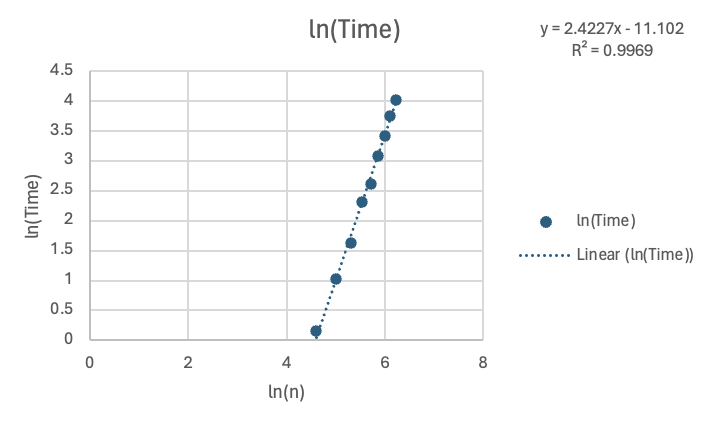
\includegraphics[width=1\linewidth]{Graphs/Matrix.png} % If the image is too large, change the "width=1" to something smaller. 
    \captionof{figure}{Matrix Determinant of $n$}

     
    
\end{minipage}\\

    The calculation of the \textit{Matrix Determinant} (unsurprisingly) involves the calculating the determinant of an $n \times n$ matrix. This algorithm utilizes \texttt{numpy.linalg.det(matrix)} in its computation, but the exact mechanism for how this algorithm finds the determinant (i.e., Gaussian elimination or other various decomposition methods [LU, QR, etc.]) is unknown. This graph has an $R^2$ score of almost exactly 1, matching the polynomial functions from Section 2.

    \subsection{Integer Factorization}

    

    \begin{minipage}{0.4\textwidth} % Sets the minipage to take up half of the page
    \centering

    
    
    \begin{tabular}{c|c|c|c}
        $n$ & $\ln(n)$ & Time(s) & $\ln(f(n))$ \\ \hline
        2 & $0.693$ & $0.012$ & $-4.345$ \\\hline
        4 & $1.386$ & $0.011$ & $-4.557$  \\\hline
        6 & $1.791$ & $0.026$ & $-3.627$\\\hline
        8 & $2.079$ & $.12$ & $-2.114$\\\hline
        10 & $2.302$ & $0.386$ & $-0.95$\\ \hline
        12 & $2.484$ & $0.717$ & $-0.331$\\ \hline
        14 & $2.639$& $1.207$ & $0.188$\\ \hline
        16 & $2.772$ & $2.43$ & $0.887$\\ \hline
        18 & $2.89$ & $6.697$ & $1.901$\\ \hline
        20 & $2.995$ & $20.01$ & $2.996$\\ \hline
        22 & $3.091$ & $38.648$ & $3.654$\\ \hline
        24 & $3.178$ & $119.084$ & $4.779$\\ \hline
        26 & $3.258$ & $169.068$ & $5.13$\\ \hline
        28 & $3.332$ & $229.562$ & $5.436$\\
    \end{tabular}
    
    \captionof{table}{\centering Integer Factorization of $n$} % Caption goes in the curly braces. Replace "Your Table Caption."
\end{minipage}%
\begin{minipage}{0.6\textwidth} % See above for reference

    

    \centering
    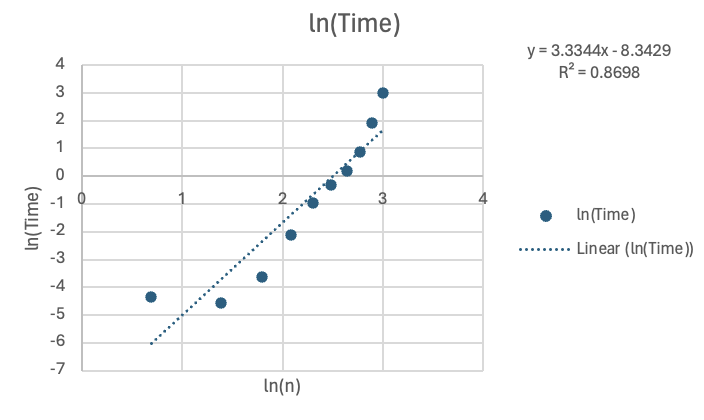
\includegraphics[width=1\linewidth]{Graphs/Integer.png} % If the image is too large, change the "width=1" to something smaller. 
    \captionof{figure}{Integer Factorization of $n$}

     
    
\end{minipage}\\

    \textit{Integer Factorization}'s graph does not have a semblance to any of the previous graphs from Section 2. A possibility for why this may be the case, is because of the skewing nature of $n = 2 \ \& \ 4$. We hypothesize that if these data points where removed, the $R^2$ value would more closely resemble that of the factorial function, or even the exponential function.



% ------------------------------------------------------------------------------
% Conclusion
% ------------------------------------------------------------------------------
    

\section{Conclusion}

    This report has extensively investigated the relationship between the size of algorithmic input, denoted as $n$, and the computational time required, represented by $t(n)$. Our analysis, reflected through detailed tables and figures, clearly demonstrates a trend where the incremental time needed to process additional elements decreases as the number of items increases. This finding not only underscores the efficiency of the algorithms analyzed but also highlights their potential scalability when applied to larger datasets.

    The implications of these results are significant, particularly in fields where large volumes of data are processed regularly. For instance, in data science and machine learning, understanding how input size affects processing time can guide the optimization of algorithms for better performance. Similarly, in software engineering, selecting the appropriate algorithm based on its performance characteristics relative to data size can enhance the responsiveness and efficiency of applications.
    
    In conclusion, the ability of an algorithm to handle increasing input sizes efficiently is crucial in our data-driven world. The insights gained from this report contribute to a deeper understanding of computational efficiency and pave the way for future research in algorithm development and optimization.
        
\newpage

% ------------------------------------------------------------------------------
% End
% ------------------------------------------------------------------------------


\end{document}
